W~celu implementacji przedstawionego algorytmu negocjacji, wykorzystaliśmy język programowania ogólnego przeznaczenia Python w~wersji 3.6 oraz bibliotekę \texttt{SPADE - Smart Python Agent Development Environment}~\cite{spade}. Biblioteka ta upraszcza proces tworzenia agentów oraz obsługuje komunikację między nimi, która oparta jest o~protokół XMPP.

\subsection{Dekompozycja systemu na agenty}
W~przygotowanym systemie możemy wydzielić dwa rodzaje agentów:
\begin{itemize}
    \item agenty zarządcze,
    \item agenty komórek fabryki. 
\end{itemize}

Na rysunku~\ref{fig:agents} przedstawiony został podział na typy agentów w~systemie.

\begin{figure}[h]
    \centering
    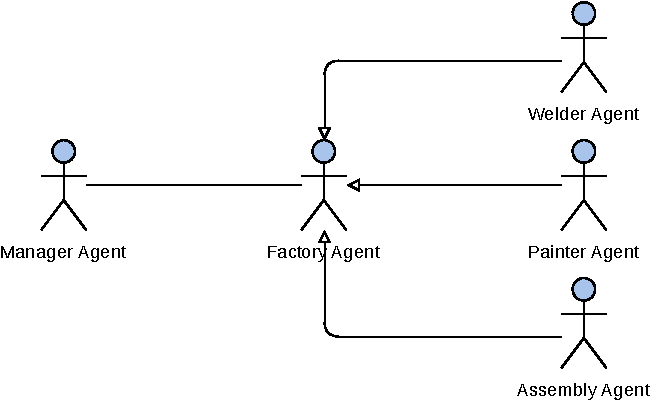
\includegraphics[width=\columnwidth]{figures/SAG-Agents.pdf}
    \caption{Dekompozycja systemu na agenty}
    \label{fig:agents}
\end{figure}

Agent \texttt{Manager Agent} zajmuje się zarządzaniem pracą w~fabryce. Do jego zadań należy:
\begin{itemize}
    \item zlecanie zadań,
    \item odbiór i~prezentacja wyników,
    \item monitorowanie działania pozostałych agentów.
\end{itemize}
W~systemie planowania pracy może znajdować się tylko jeden agent tego typu. Zarządca jest elementem krytycznym systemu, jego uszkodzenie powoduje błąd całego systemu.

Agent \texttt{Factory Agent} reprezentuje pojedynczą komórkę roboczą fabryki. To właśnie one realizują postawione zadanie planowania. Zadaniem agentów tego typu jest:
\begin{itemize}
    \item (pareto) optymalizacja lokalna sekwencji,
    \item negocjowanie z~innymi agentami tego typu,
    \item zgłaszanie problemów z~komunikacją do zarządcy.
\end{itemize}

W~celu prezentacji działania algorytmu zdecydowaliśmy się na stworzenie trzech oddzielnych komórek fabryki, reprezentowanych przez:
\begin{itemize}
    \item agenta spawalni \texttt{Welder Agent},
    \item agenta lakierni \texttt{Painter Agent},
    \item agenta stacji montażowej \texttt{Assembly Agent}.
\end{itemize}

\subsection{Dekompozycja agentów na zachowania}
Każdy agent składa się z~kilku zachowań działających współbieżnie. Zachowanie jest zadaniem, które agent może realizować w~powtarzalny sposób. Biblioteka \texttt{SPADE}~\cite{spade} udostępnia podstawowe typy zachowań:
\begin{itemize}
    \item \texttt{One-Shot} - jednorazowe zachowanie,
    \item \texttt{Cyclic} - cyklicznie uruchamiane zachowanie,
    \item \texttt{Timeout} - jednorazowe zachowanie, uruchamiane przez agenta w~wyszczególnionej chwili czasowej,
    \item \texttt{FSM} - umożliwia definiowanie zachowania przy użyciu skończonego automatu stanów.
\end{itemize}

Z~każdym zachowaniem, skojarzony jest szablon wiadomości. W~momencie przyjścia wiadomości, dla każdego zachowania, agent sprawdza czy wiadomość jest zgodna z~szablonem. Jeżeli wiadomość i~szablon, są ze sobą zgodne, to agent umieszcza wiadomość w~skrzynce odbiorczej danego zachowania, z~którego może ona zostać pobrana. 

\todo{Tu opisać zachowania menedżera}

\todo{Tu opisać zachowania fabryki}